\documentclass[11pt]{article}

\usepackage{graphicx}
\usepackage[top=25mm, bottom=25mm, left=25mm, right=25mm, a4paper]{geometry}
\usepackage{amsmath}
\usepackage{enumitem}
\usepackage{float}
\usepackage{fancyhdr}
\usepackage{booktabs}
\usepackage{tikz}
\usepackage{steinmetz}
\usepackage{pgfplots}

\pagestyle{fancy}
\fancyhf{}
\fancyhead[R]{Baturay Kafkas - 2240357068 - Electrical \& Electronics Engineering}

\rfoot{\thepage}
\renewcommand{\headrulewidth}{0pt} 
\renewcommand{\footrulewidth}{0pt}
\sloppy

\begin{document}

\begin{center}
\large
\textbf{ELE214 - Electronics Laboratory I Preliminary Work 1}
\end{center}

\section{Questions}

\begin{enumerate}[leftmargin=*,label=\textbf{\arabic*.}]

\item How can a semiconductor diode be tested for defects by means of an ohmmeter?

\item Draw the I-V characteristics of a semiconductor diode and indicate all the critical points on the plot. Explain the difference between germanium and silicon diodes, considering their I-V characteristics.

\item Design a half-wave rectifier circuit that has 220 V$_{\text{rms}}$ AC signal with 50 Hz as input and supplies 5.40 V$_{\text{DC}}$ to a purely resistive load. Assume that circuit elements are ideal.

\item If a capacitor is connected in parallel to the resistive load in the previous circuit, how will the ripple voltage and mean output voltage change? Plot the load voltage for one period.

\item Repeat questions 3 and 4 for the full-wave rectifier circuit.

\end{enumerate}

\textbf{Experimental Work (Simulation of 2-5)}

\begin{enumerate}[leftmargin=*,label=\textbf{\arabic*.}]

\item By using an avometer, check the semiconductor diodes. Measure and record the values of $V_f$ (forward bias voltage) and $V_r$ (reverse bias voltage) of each diode. 

\item Set up the circuit in the following figure. Observe the characteristics curve of the diode on oscilloscope and plot it. Find the value of the threshold voltage $V_o$.

\begin{figure}[H]
    \centering
    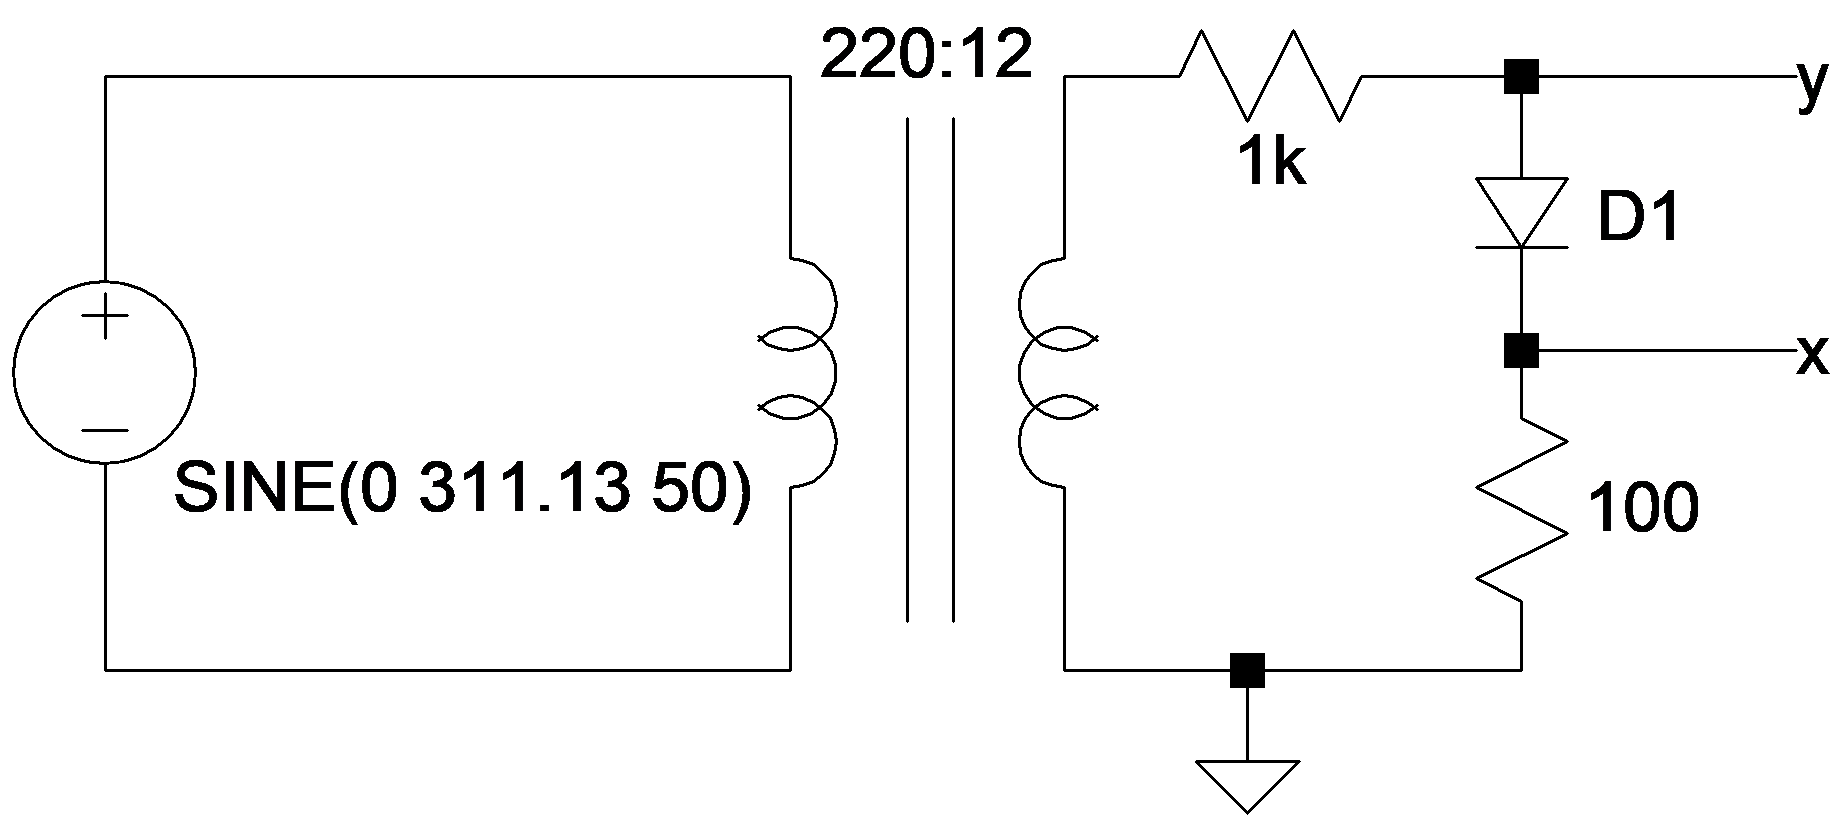
\includegraphics[width=0.65\linewidth]{q2_s.png}
\end{figure}

\item Set up the circuit designed in preliminary work Question 3 with using a load resistance of $R_L=1\:k\Omega$. Observe and plot the output voltage waveform. Measure the mean values of $V_o$ and $I_o$ using an avometer.

\item Connect a capacitor $C_1=100$ $\:\mu$F in parallel to the load of the circuit in Question 3. Observe and plot the output voltage waveform. Measure the peak to peak value of ripple voltage $V_r$. Measure the mean value of $V_o$ using an avometer. Repeat for a capacitor $C_2=1$ mF.

\item Repeat Question 4 for the full wave rectifier designed in preliminary work.

\end{enumerate}

\section{Answers}

\begin{enumerate}[leftmargin=*,label=\textbf{\arabic*.}]

\item To observe whether the diode is defective, we determine the behavior of the diode when it is forward- or reverse-biased.

At first, connect the positive lead to the anode and the negative lead to the cathode. If the meter shows a high impedance reading, the diode effectively acts as an open circuit, which is an unintended behavior.

Second, do the vice versa. If the meter shows a low impedance reading, the diode effectively acts as a short circuit, which is also unintended.

\item Let us plot the I-V characteristics of the silicon and germanium diodes and compare the differences.
\begin{center}
\begin{minipage}{0.48\textwidth}
\centering
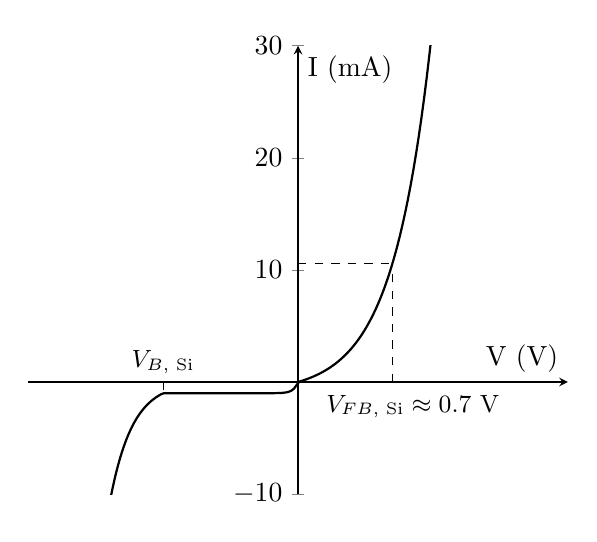
\begin{tikzpicture}
\begin{axis}[
    xlabel={V (V)},
    ylabel={I (mA)},
    xmin=-2, xmax=2,
    ymin=-10, ymax=30,
    axis lines=middle,
    xtick=\empty,
]

% Silicon diode
\addplot[
    domain=-2:2,
    samples=200,
    thick
]
{ x < 0 ? (x < -1 ? 1/e^6*(-e^(-6*x)) : e^(30*x)-1) : exp(3.5*x) - 1 };

\draw[dashed] (axis cs: 0.7, 0) -- (axis cs: 0.7, 10.59) (axis cs: 0, 10.59) -- (axis cs: 0.7, 10.59) (axis cs: -1, 0) -- (axis cs: -1,-1);

\node at (axis cs: 0.85, -2.2) {\small $V_{FB,\text{ Si}}\approx 0.7$ V};
\node at (axis cs: -1, 1.8) {\small $V_{B,\text{ Si}}$};

\end{axis}
\end{tikzpicture}

\small \textit{Graph 1: Silicon diode I--V characteristics}
\end{minipage}\hfill\begin{minipage}{0.48\textwidth}
\centering
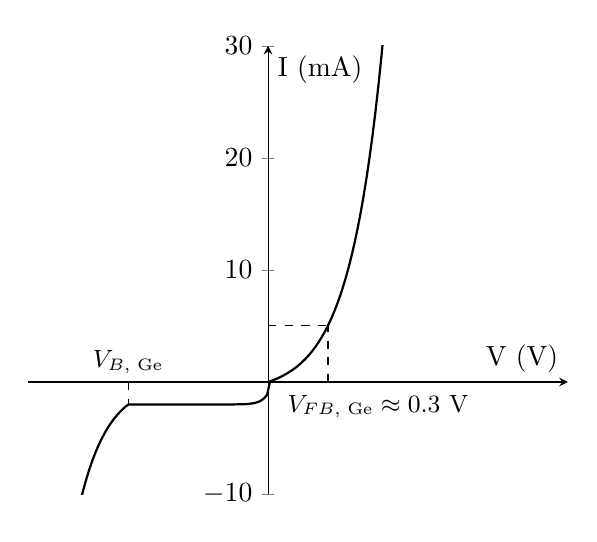
\begin{tikzpicture}
\begin{axis}[
    xlabel={V (V)},
    ylabel={I (mA)},
    xmin=-1.2, xmax=1.5,
    ymin=-10, ymax=30,
    axis lines=middle,
    xtick=\empty,
]

\draw[dashed] (axis cs: 0.3, 0) -- (axis cs: 0.3, 5.05) (axis cs: 0, 5.05) -- (axis cs: 0.3, 5.05) (axis cs: -0.7, 0) -- (axis cs: -0.7,-2);

\node at (axis cs: 0.55, -2.2) {\small $V_{FB,\text{ Ge}}\approx 0.3$ V};
\node at (axis cs: -0.7, 1.8) {\small $V_{B,\text{ Ge}}$};

% Germanium diode
\addplot[
    domain=-1:2,
    samples=200,
    thick
]
{ x < 0 ? (x < -0.7 ? 2/e^4.9*(-e^(-7*x)) : min(e^(30*x)-2, 40)) : min(exp(6*x), 40) - 1};

\end{axis}

\end{tikzpicture}

\small \textit{Graph 2: Germanium diode I--V characteristics}
\end{minipage}

\end{center}

\begin{center}
\begin{tabular}{|c|c|c|}
\hline
\textbf{Property} & \textbf{Silicon Diode (Si)} & \textbf{Germanium Diode (Ge)} \\
\hline
Forward voltage & $\approx 0.7~\mathrm{V}$ & $\approx 0.3~\mathrm{V}$ \\\hline
Reverse leakage current & Very small (nA) & Higher (µA) \\\hline
Temperature stability & Better & Poorer \\\hline
Reverse breakdown tolerance & Generally higher & Generally lower \\\hline
\end{tabular}
\end{center}

\item To obtain $5.40 $ V$_\text{DC}$, the peak voltage across the resistor should be $\pi$ times V$_\text{DC}$.
\[V_p=5.40\cdot\pi\]

The diode is ideal. Therefore, the voltage across the secondary terminals of the transformer is also $V_p$. The peak voltage supplied by the AC signal is $220\sqrt2$. From the ideal transformer equation,
\[\frac{V_1}{N_1}=\frac{V_2}{N_2},\]

where $V_1=220\sqrt2$ and $V_2=5.40\cdot\pi$. Substituting the numerical values, the ratio $\frac{N_1}{N_2}$ becomes
\[\frac{N_1}{N_2}=\frac{V_1}{V_2}=\frac{220\sqrt2}{5.40\cdot\pi}\approx18.34\implies\frac{N_1}{N_2}\approx\frac{55}{3}.\]

The inductance ratio then becomes
\[\frac{L_1}{L_2}=\left(\frac{N_1}{N_2}\right)^2=\frac{55^2}{3^2}=\frac{3025}{9}.\]

\begin{figure}[H]
    \centering
    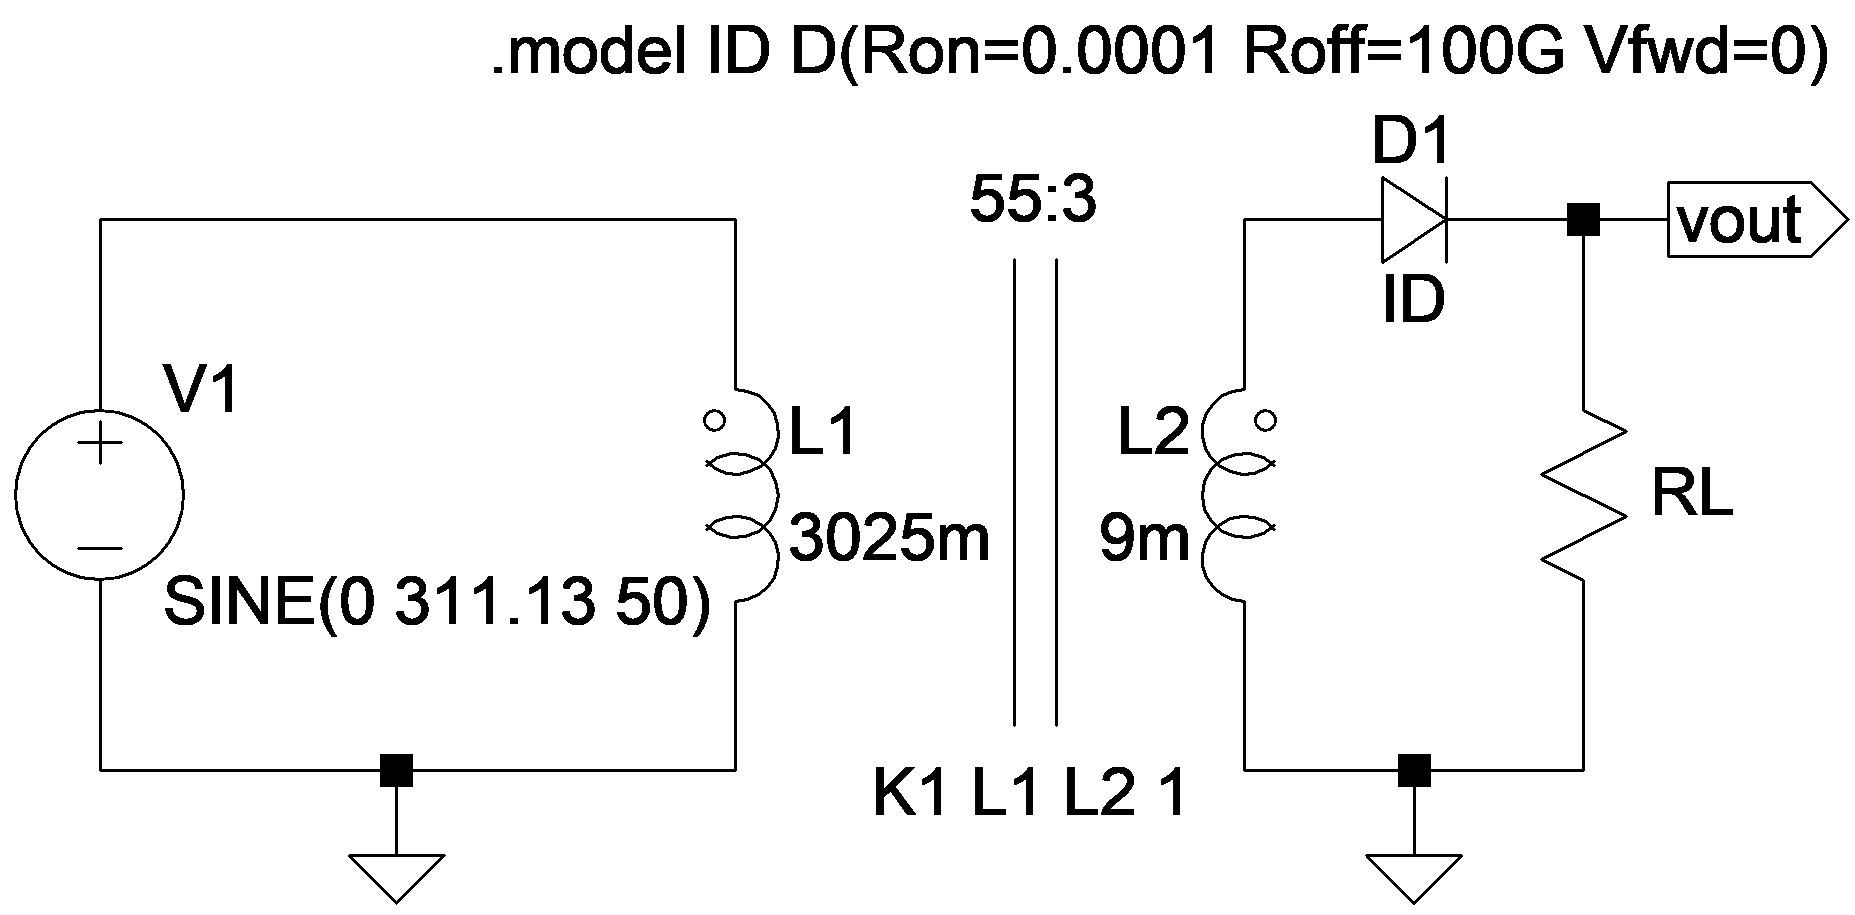
\includegraphics[width=0.65\linewidth]{q3.png}

    \textit{Circuit 1}
\end{figure}

\item Adding a capacitor in parallel with the resistor obviates the ripple voltage significantly. $V_\text{out}$ is also higher compared to in Question 3 because the area under the $V_\text{out}$ curve increases as a result of the capacitor being connected.

The circuit with $C=0.1\:\mu$F and $ R=1\: k\Omega$ is given.

\begin{figure}[H]
    \centering
    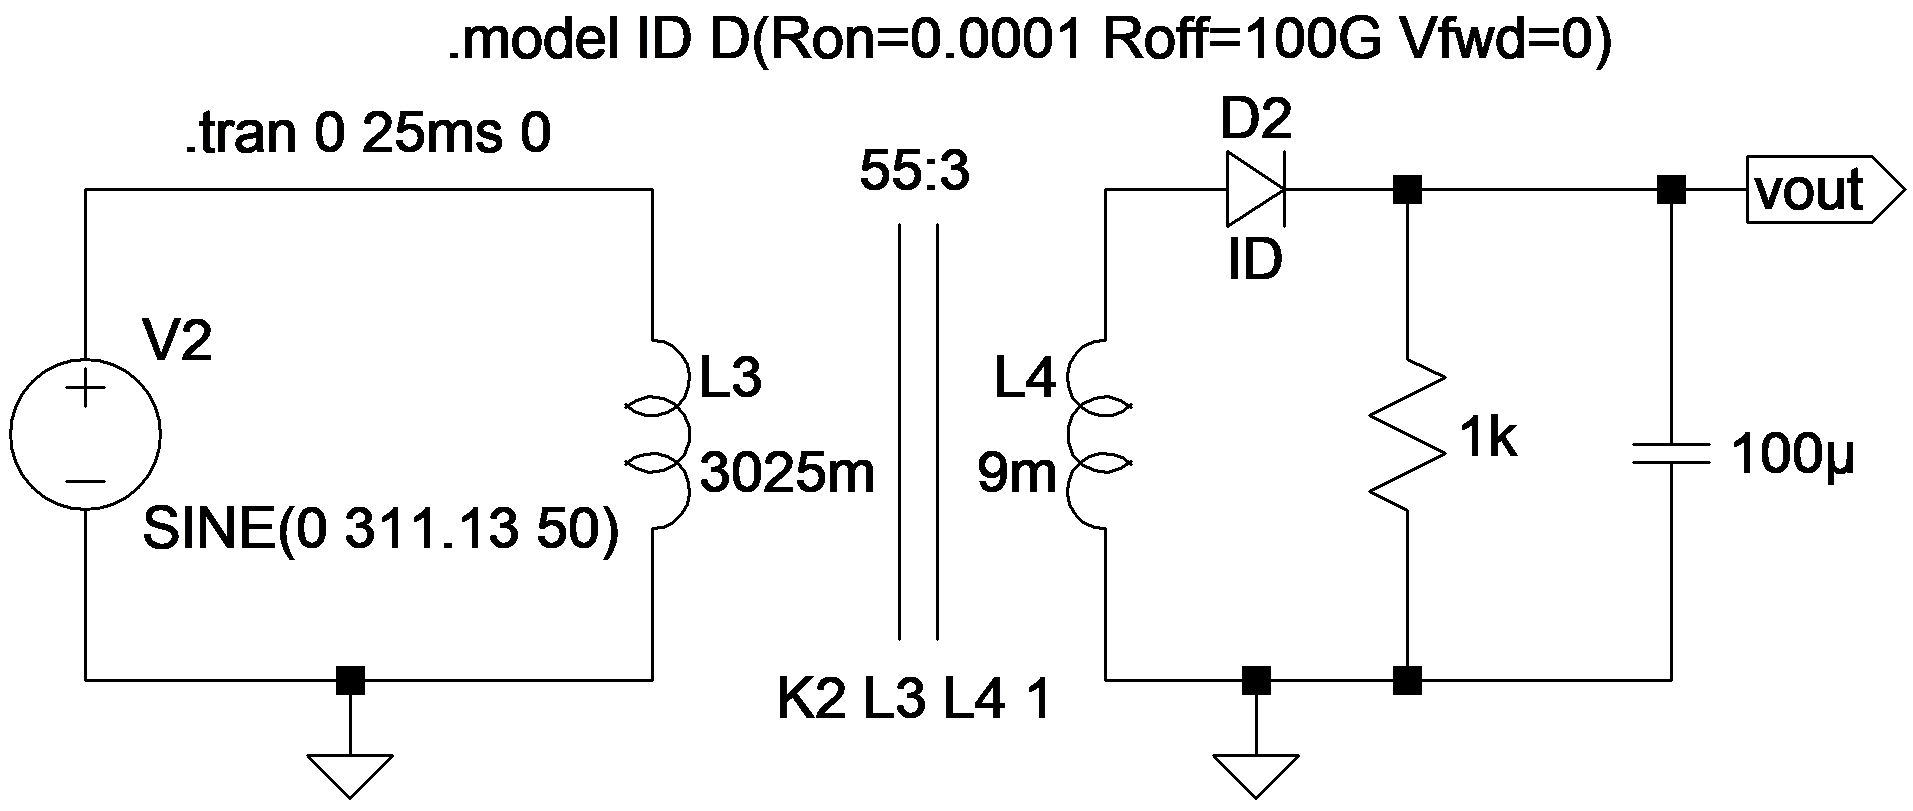
\includegraphics[width=0.8\linewidth]{q4.png}

    \textit{Circuit 2}
\end{figure}

\begin{figure}[H]
    \centering
    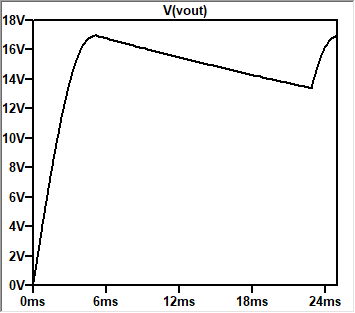
\includegraphics[width=0.4\linewidth]{LTspice_erCpSfLG49.png}

    \textit{Graph 3: One-period plotting of Circuit 2}
\end{figure}

\newpage

\item The peak voltage across the resistor should be $\pi\over2$ times V$_\text{DC}$ now.
\[V_p=5.40\cdot\pi\cdot\frac12\]

Calculations give
\[\frac{N_1}{N_2}=\frac{V_1}{V_2}=\frac{220\sqrt2}{5.40\cdot\pi\cdot \frac12}\approx36.68\implies\frac{N_1}{N_2}\approx\frac{110}{3},\]
\[\frac{L_1}{L_2}=\left(\frac{N_1}{N_2}\right)^2=\frac{110^2}{3^2}=\frac{12100}{9}\]

\begin{figure}[H]
    \centering
    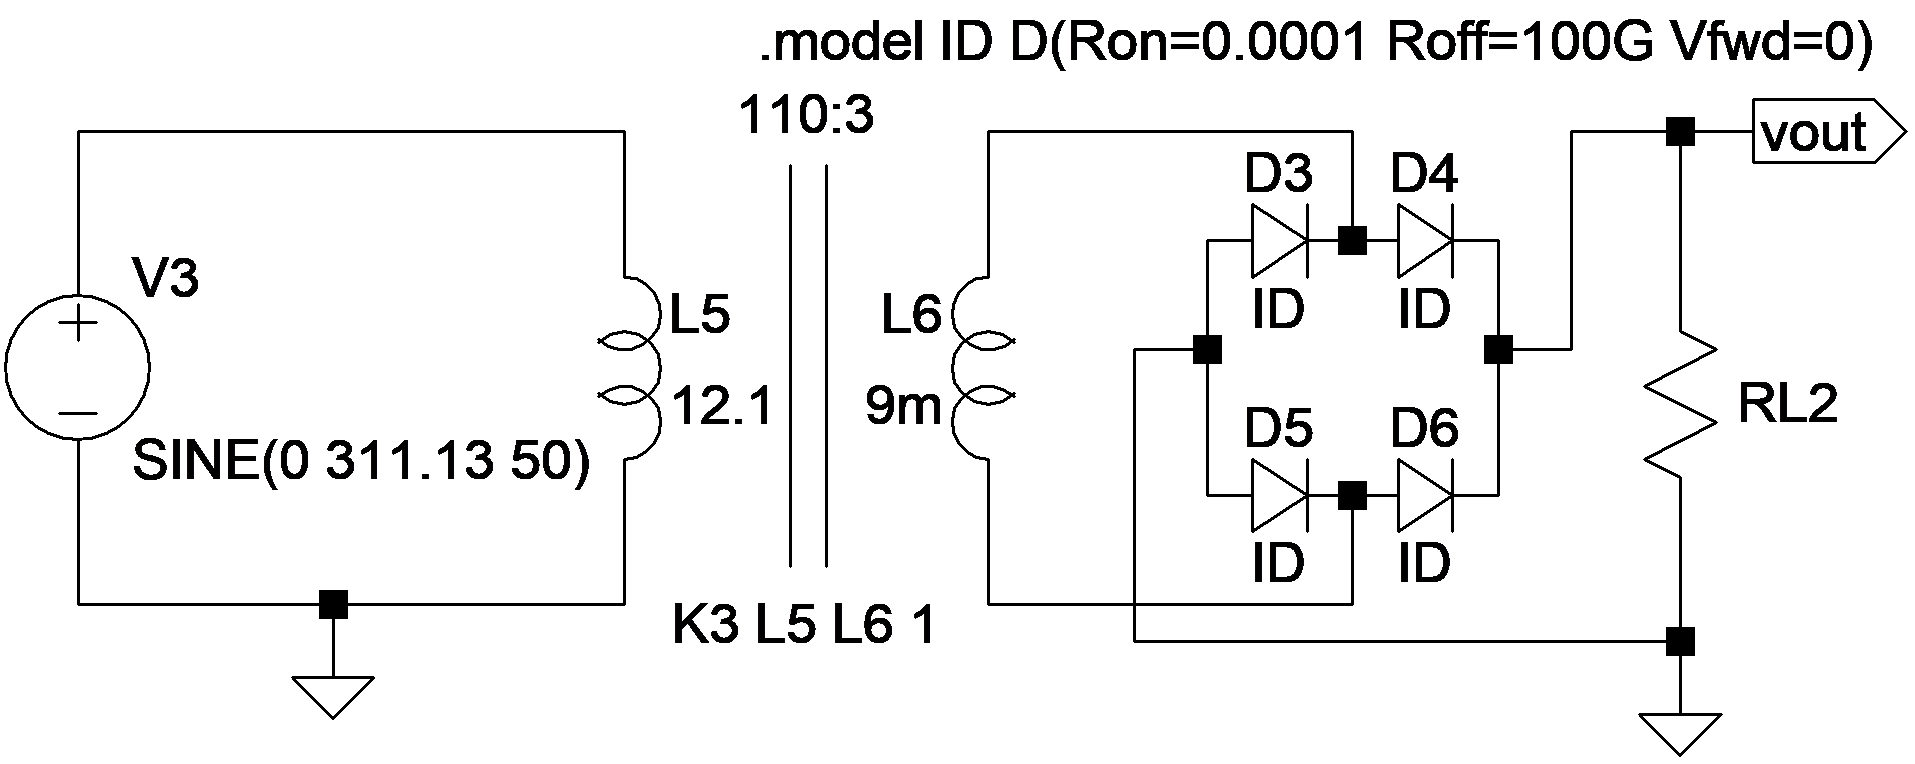
\includegraphics[width=0.8\linewidth]{q5_1.png}

    \textit{Circuit 3}
\end{figure}

The circuit with $C=0.1\:\mu$F and $ R=1\: k\Omega$:

\begin{figure}[H]
    \centering
    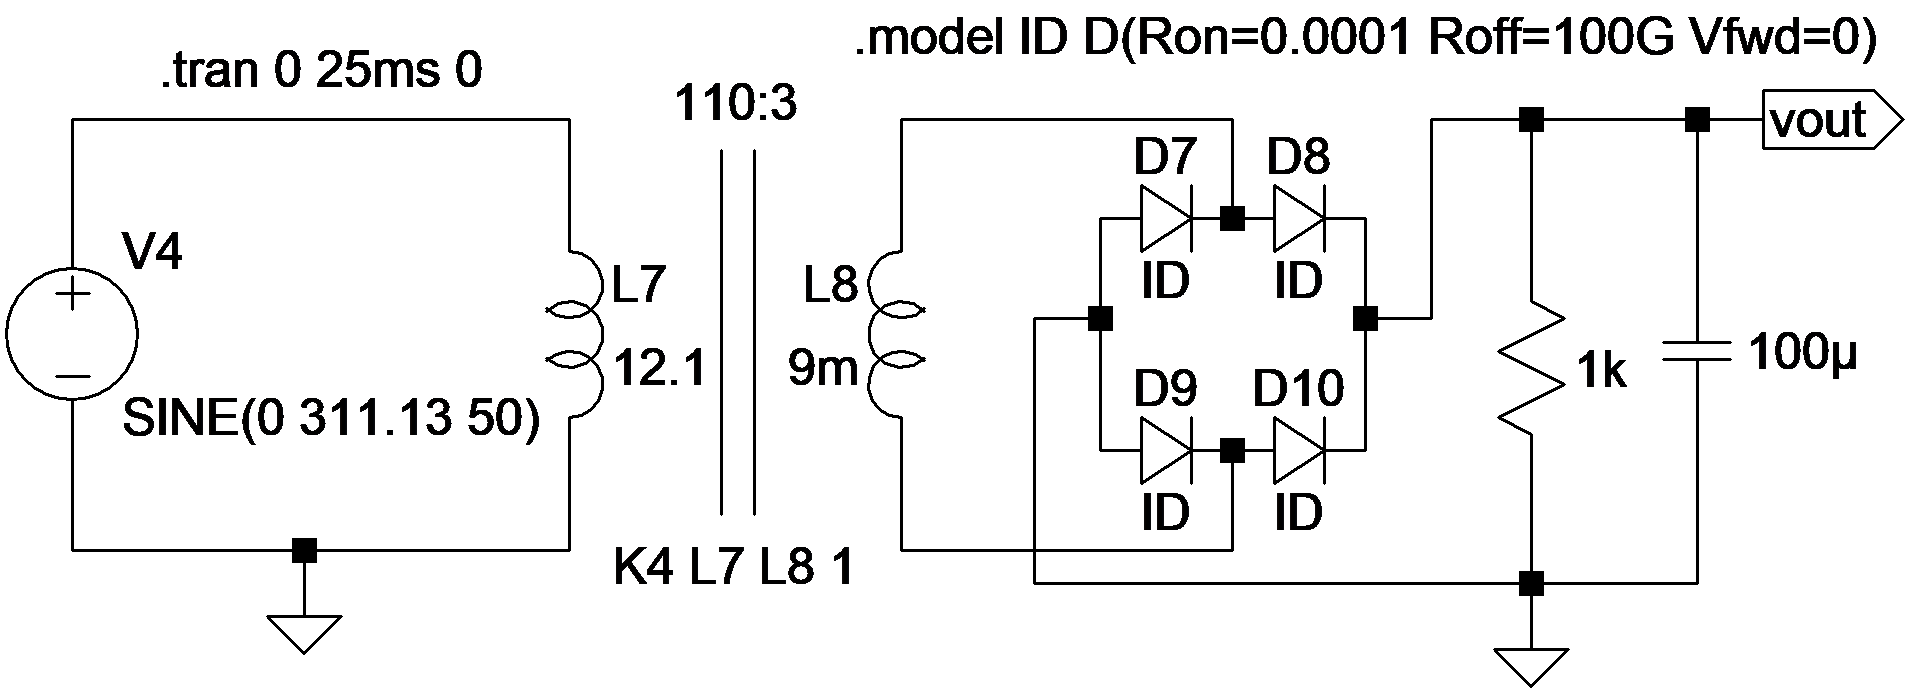
\includegraphics[width=0.85\linewidth]{q5_2.png}

    \textit{Circuit 4}
\end{figure}

\begin{figure}[H]
    \centering
    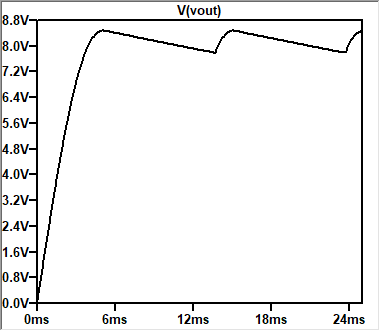
\includegraphics[width=0.4\linewidth]{LTspice_LG6K7XhC8G.png}

    \textit{Graph 4: One-period plotting of Circuit 4}
\end{figure}

\end{enumerate}

\newpage

\textbf{Simulation}

\begin{enumerate}[leftmargin=*,label=\textbf{\arabic*.}]
\setcounter{enumi}{1}

\item The circuit and the graph of the voltage across the diode are below.

\begin{figure}[H]
    \centering
    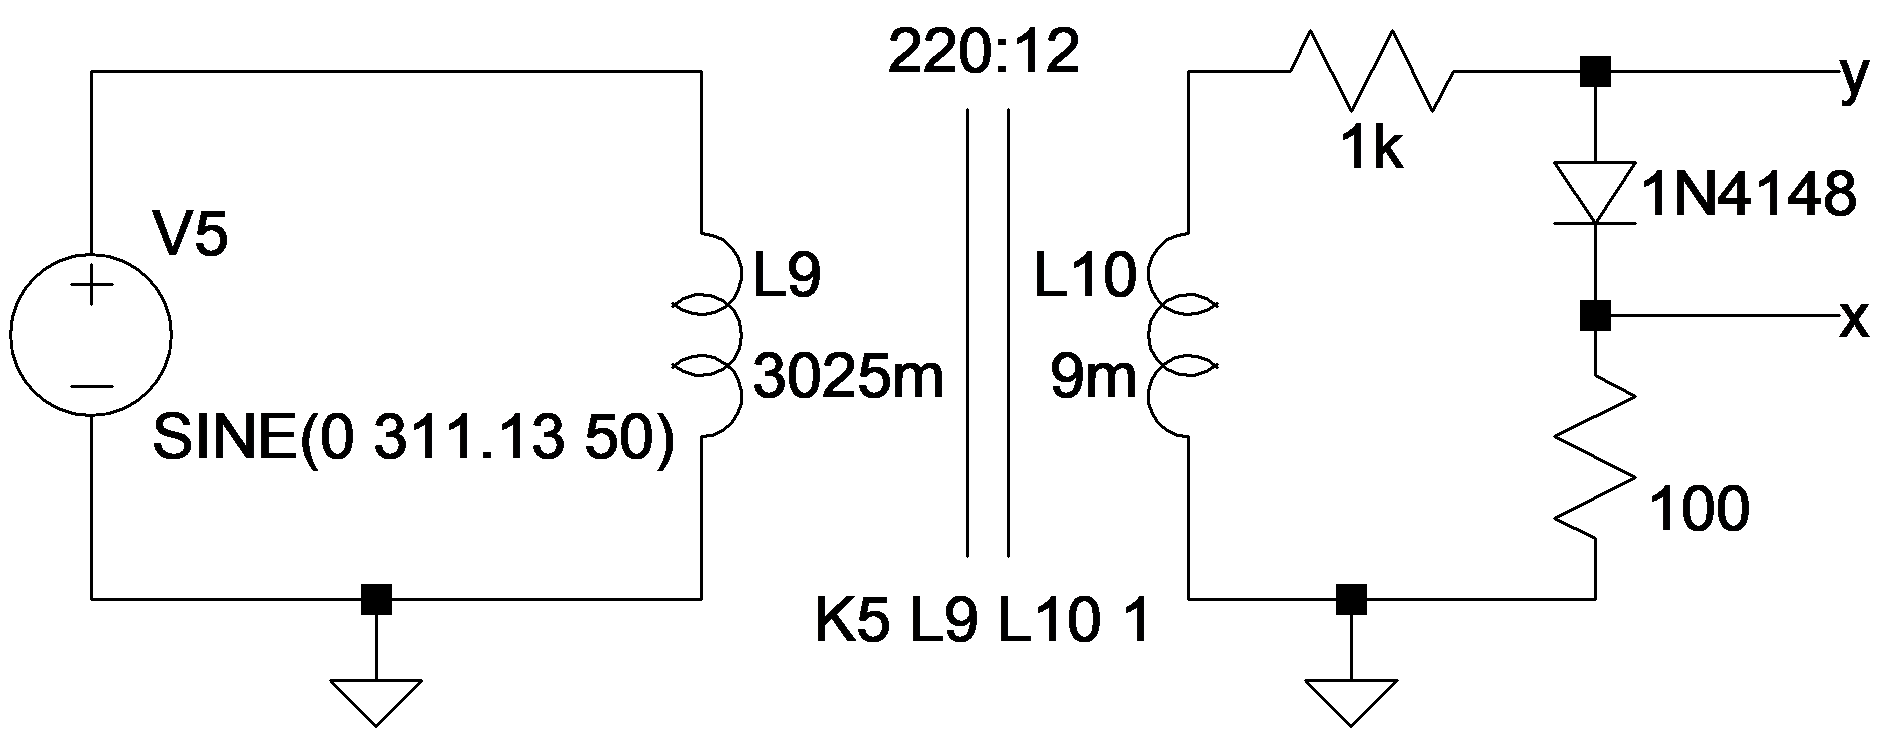
\includegraphics[width=0.8\linewidth]{q2_sa.png}

    \textit{Circuit 5}
\end{figure}

\begin{minipage}{0.48\textwidth}
\begin{figure}[H]
    \centering
    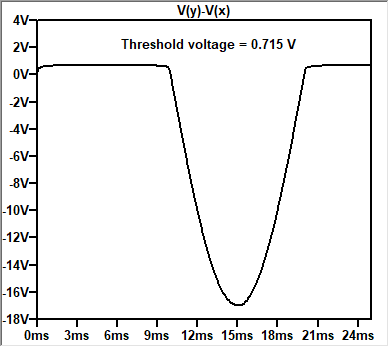
\includegraphics[width=0.8\linewidth]{LTspice_KJL4pP6efh.png}

    \textit{Graph 5: The voltage across the diode in Circuit 5}
\end{figure}
\end{minipage}\hfill\begin{minipage}{0.48\textwidth}
\begin{figure}[H]
    \centering
    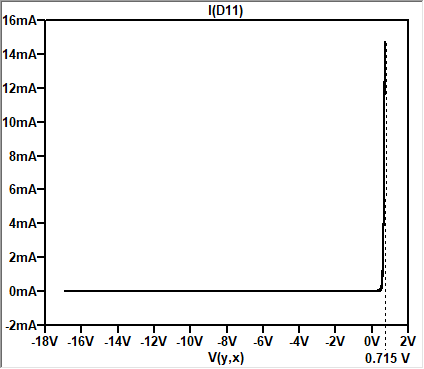
\includegraphics[width=0.8\linewidth]{LTspice_p7lwX1jvvk.png}

    \textit{Graph 6: The I-V characteristics of the diode in Circuit 5}
\end{figure}
\end{minipage}

\vspace{1em}

We can infer from the graph that the forward bias voltage may deviate from the known value.

\item The ideal diode is now replaced by a silicon diode with $V_{FB}=0.7$ V.

\begin{figure}[H]
    \centering
    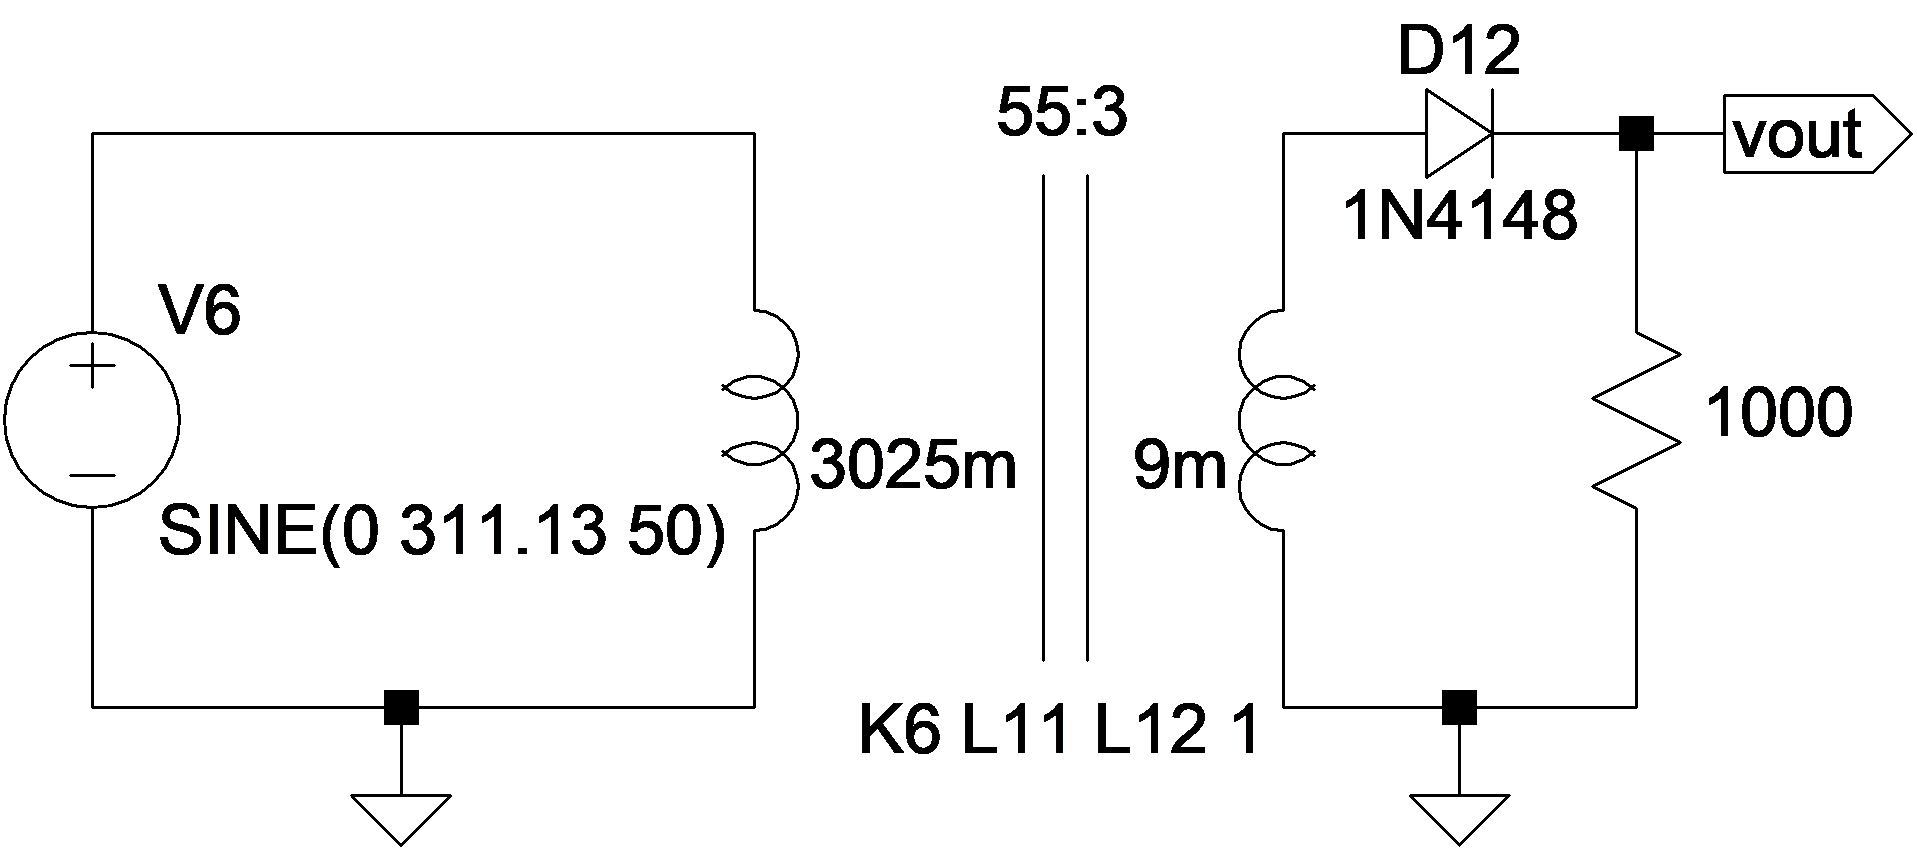
\includegraphics[width=0.7\linewidth]{q3_s.png}
    
    \textit{Circuit 6}
\end{figure}

\begin{figure}[H]
    \centering
    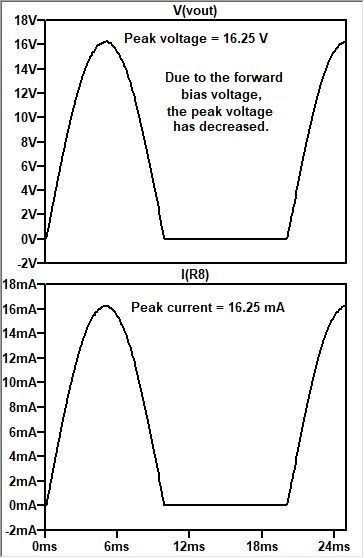
\includegraphics[width=0.4\linewidth]{LTspice_Koy00PIfnD.png}

    \textit{Graphs 7 and 8: The voltage across and the current through the resistor in Circuit 6}
\end{figure}
\[V_m=\frac{V_p}{\pi}=5.17\text{ V}\qquad I_m=\frac{I_p}{\pi}=5.17\text{ mA}\]

\item The circuits and the graphs are as follows.

\begin{figure}[H]
    \centering
    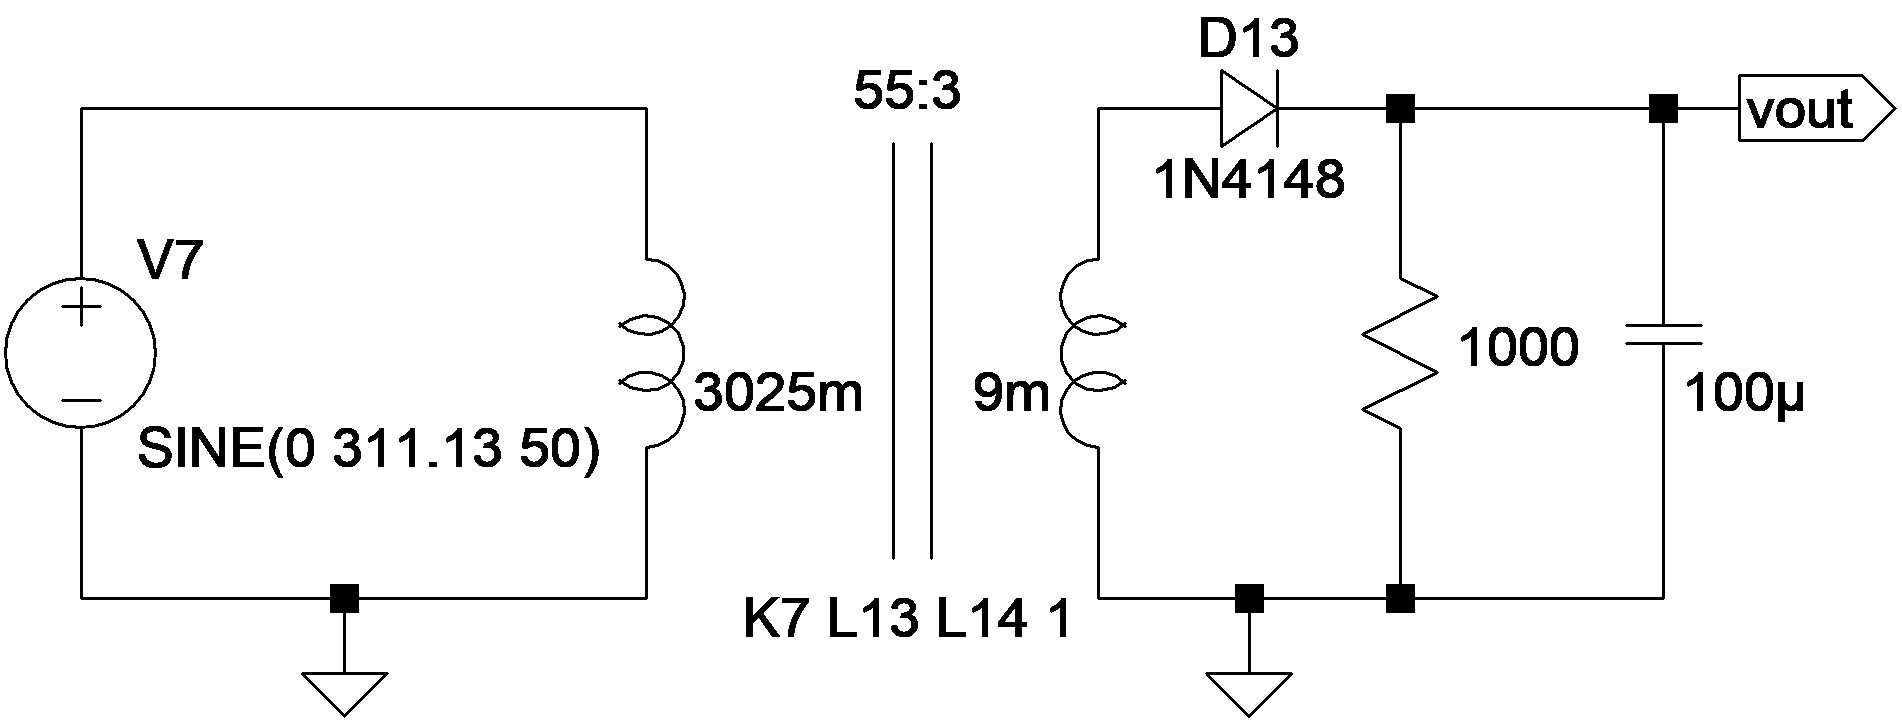
\includegraphics[width=0.75\linewidth]{q4_s1.png}
    
    \textit{Circuit 7 with} $100\:\mu\text{F}$ \textit{capacitor}

    \vspace{1em}
    
    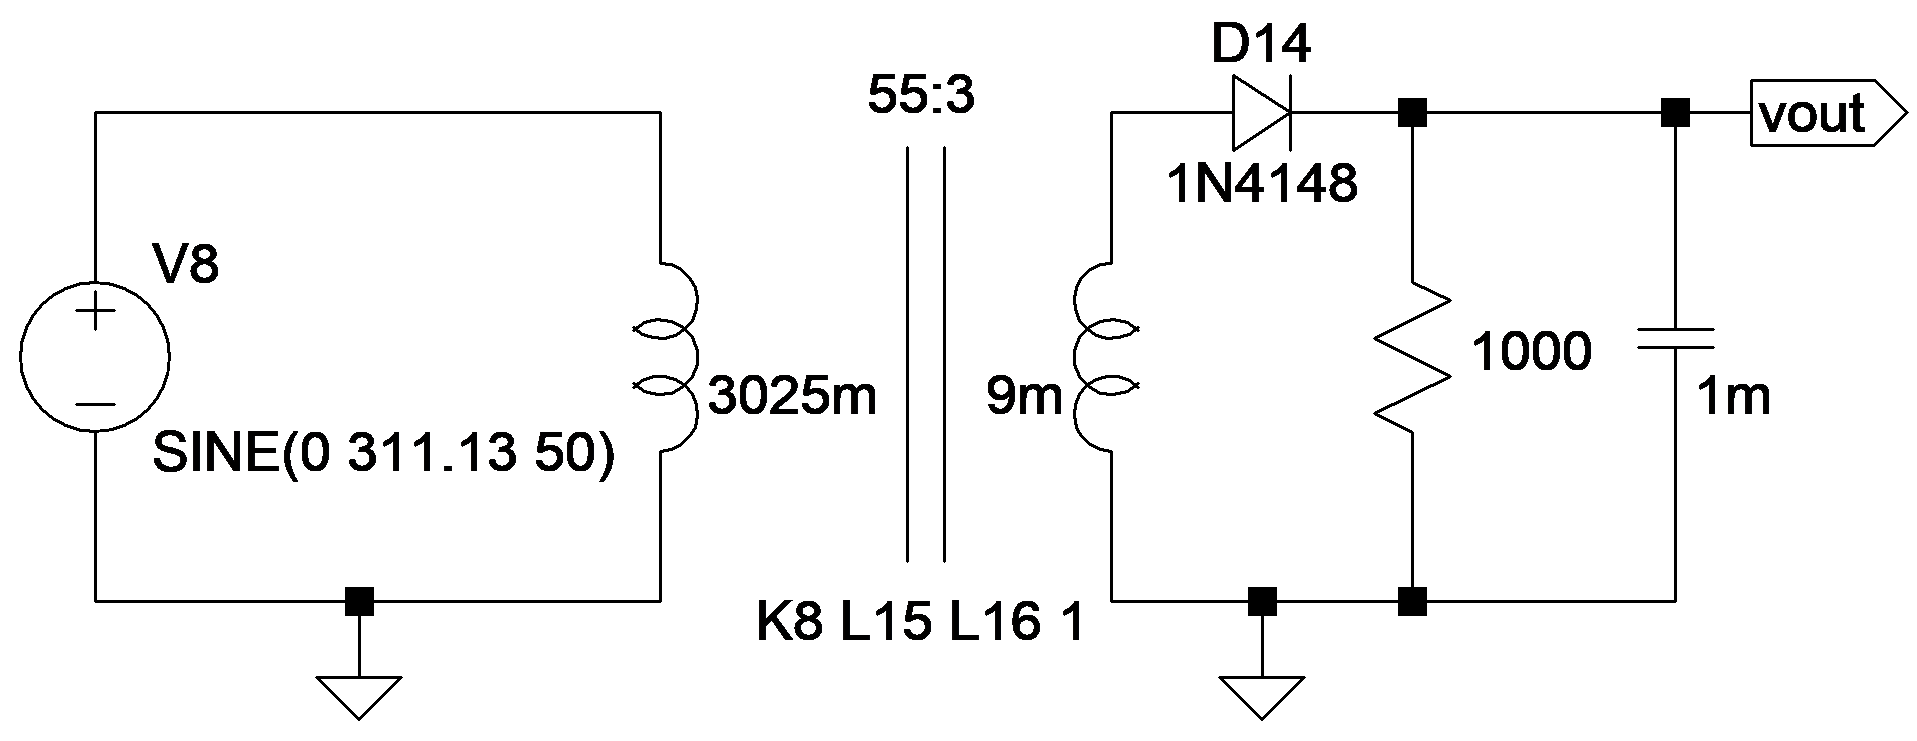
\includegraphics[width=0.75\linewidth]{q4_s2.png}
    
    \textit{Circuit 8 with} $1000\:\mu\text{F}$ \textit{capacitor}
\end{figure}

\newpage

\begin{minipage}{0.48\textwidth}
\begin{figure}[H]
    \centering
    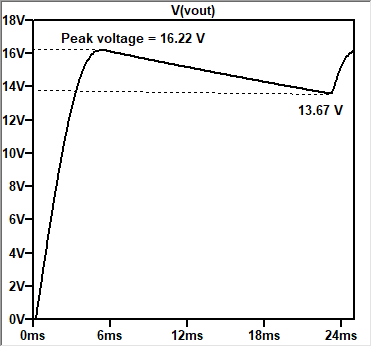
\includegraphics[width=0.8\linewidth]{LTspice_UONrn6N8Zb.png}
    
    \textit{Graph 9: Circuit 7 for one period}
    \[V_R=16.22-13.67=2.55\text{ V}\]
    Mean value of $V_o$:\\[0.5em] $V_o\approx V_p-\frac{V_R}2=16.22-\frac{2.55}2\approx14.95\text{ V}$.
\end{figure}
\end{minipage}\hfill\begin{minipage}{0.48\textwidth}
\begin{figure}[H]
    \centering
    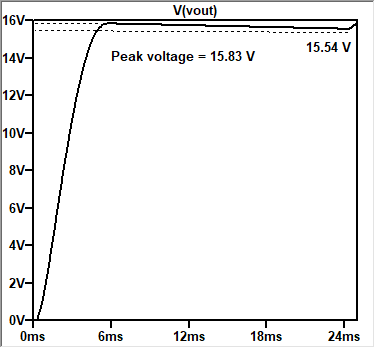
\includegraphics[width=0.8\linewidth]{LTspice_TZtZPmR2f8.png}

    \textit{Graph 10: Circuit 8 for one period}
    \[V_R=15.83-15.54=0.29\text{ V}\]
    Mean value of $V_o$:\\[0.5em] $V_o\approx V_p-\frac{V_R}2=15.83-\frac{0.29}2\approx15.69\text{ V}$.
\end{figure}
\end{minipage}

\item The circuits and the graphs are as follows.

\begin{figure}[H]
    \centering
    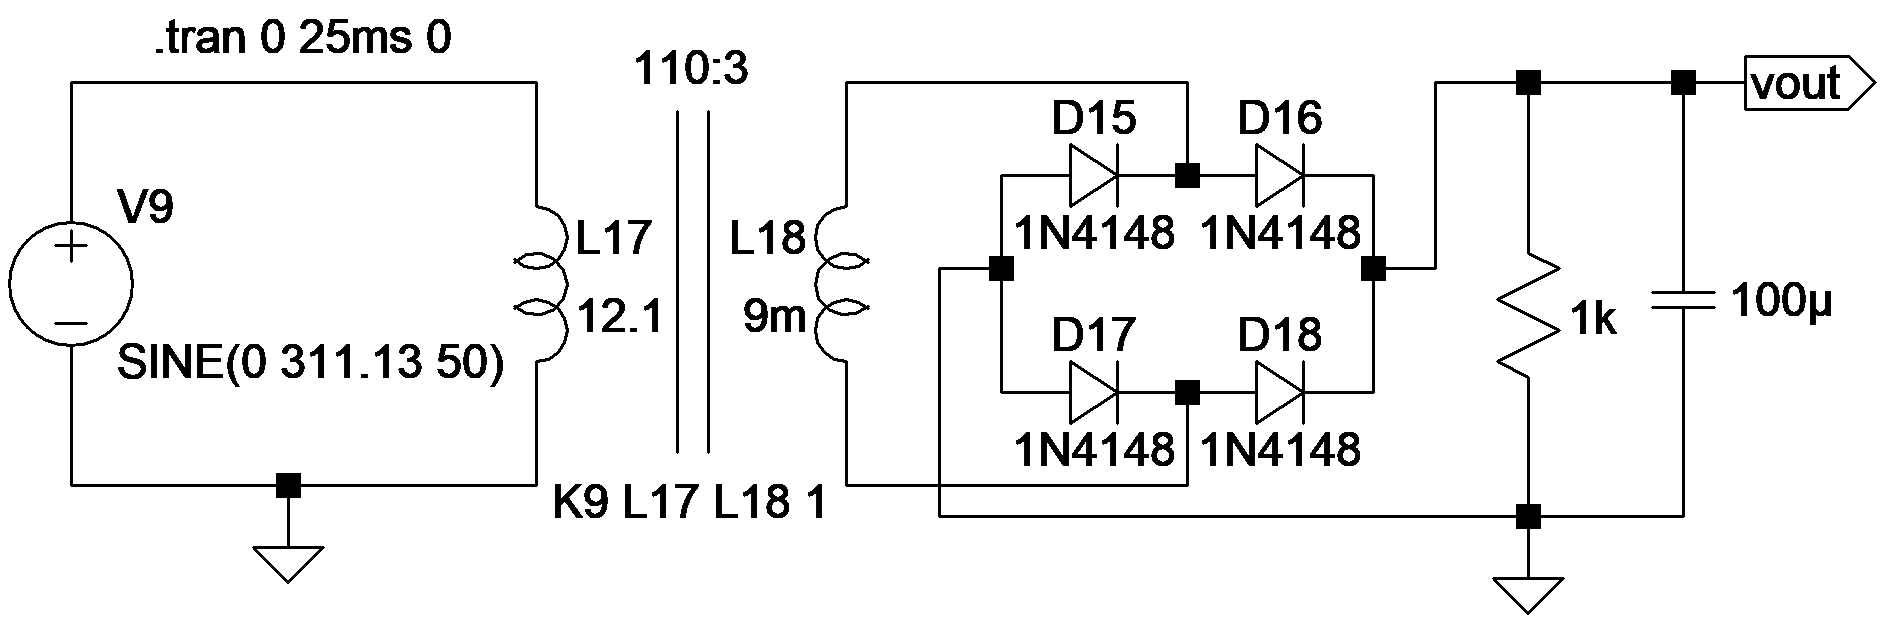
\includegraphics[width=0.85\linewidth]{q5_s1.png}
    
    \textit{Circuit 9 with} $100\:\mu\text{F}$ \textit{capacitor}

    \vspace{1em}
    
    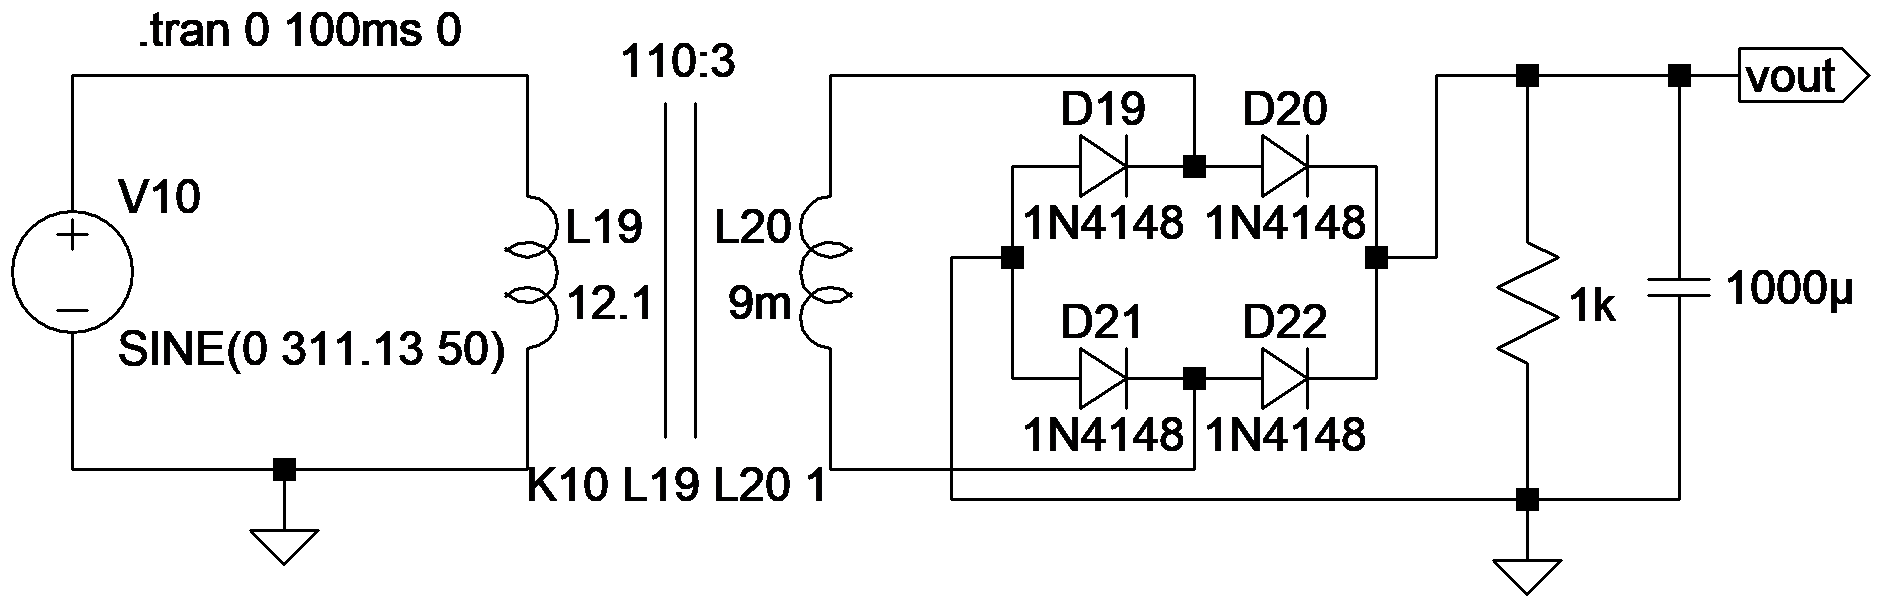
\includegraphics[width=0.85\linewidth]{q5_s2.png}
    
    \textit{Circuit 10 with} $1000\:\mu\text{F}$ \textit{capacitor}
\end{figure}

\begin{minipage}{0.48\textwidth}
\begin{figure}[H]
    \centering
    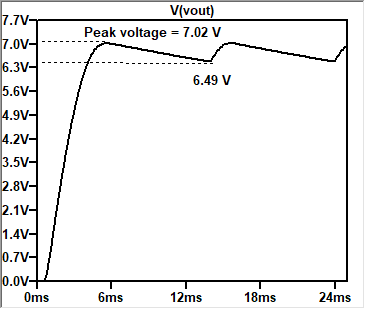
\includegraphics[width=0.8\linewidth]{LTspice_Su3surXYhw.png}

    \textit{Graph 11: Circuit 9 for one period}
    \[V_R=7.02-6.49=0.53\text{ V}\]
    Mean value of $V_o$:\\[0.5em] $V_o\approx V_p-\frac{V_R}2=7.02-\frac{0.53}2\approx6.76\text{ V}$.
\end{figure}
\end{minipage}\hfill\begin{minipage}{0.48\textwidth}
\begin{figure}[H]
    \centering
    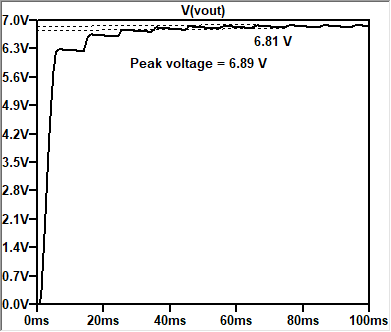
\includegraphics[width=0.8\linewidth]{LTspice_dgTgIDFElz.png}

    \textit{Graph 12: Circuit 10 for four periods}
    \[V_R=6.89-6.81=0.08\text{ V}\]
    Mean value of $V_o$:\\[0.5em] $V_o\approx V_p-\frac{V_R}2=6.89-\frac{0.08}2=6.85\text{ V}$.
\end{figure}
\end{minipage}
\end{enumerate}

\end{document}